%----------------------------------------------------------------
%
%  File    :  chapter2.tex
%
%  Authors :  Keith Andrews, IICM, TU Graz, Austria
%             Manuel Koschuch, FH Campus Wien, Austria
% 
%  Created :  22 Feb 96
% 
%  Changed :  30 Oct 2008
%  !TEX root = ./thesis.tex
%----------------------------------------------------------------


\chapter{Xamarin als Cross-Platform Framework}
\label{chap:xamarin}
	Xamarin ist ursprünglich als Firma Xamarin 2011 von Mono Entwicklern gegründet und 2016 von Microsoft übernommen worden. Microsoft hat Xamarin weiterentwickelt und stellt es heute als Open-Source Cross-platform Framework für Visual Studio ab Version 2015 und für Mac als Visual Studio for Mac zur Verfügung. Mit diesem Framework kann eine Cross-platform Applikation für Android, iOS und Windows 10 (früher Windows Mobile) geschrieben werden.

	\textbf{Mono} ist eine Software Plattform die es ermöglicht Cross-platform Applikationen bzw. Software unter Einbindung von Microsofts .NET Framework zu entwickeln. Es basiert auf C\# als Programmiersprache und ist eine plattformunabhängige Software. Programme die in .NET geschrieben wurden und auf einem Linux Kernel ausgeführt werden sollen, greifen auf Mono zurück um dies zu ermöglichen. Mono bildet somit eine Schnittstelle um Microsofts .NET Framework zu verwenden.

	\textbf{Das .NET Framework} wiederum ist eine, ursprünglich von Microsoft entwickelte Softwareentwicklungsplattform, die in direkter Konkurrenz zu JAVA SE und JAVA EE steht. Es stellt eine Laufzeitumgebung (Common Language Runtime) für auszuführende Programme zur Verfügung und ermöglicht das Einbinden einer Vielzahl von Klassenbibliotheken und Programmierschnittstellen.

	Wird eine .NET Anwendung ausgeführt so ist zum Kompilierungszeitpunkt eine Übersetzung in eine Zwischensprache (Common Intermediate Language) notwendig. Anschließend wird das Kompilat von der .NET Laufzeitumgebung in die Maschinensprache des Zielsystems übersetzt und ausgeführt. Diese Übersetzung aus der Common Intermediate Language geschieht durch den sogenannten Just-In-Time Compiler (JIT) - welcher bei Xamarin.Android verwendet wird um die Anwendung für das Android Betriebssystem zu erstellen. Eine iOS Anwendung unterstützt diesen JIT nicht. Die iOS Anwendung wird in Intermediate Language (IL) kompiliert und anschließend mittels eines Apple Compilers (Ahead-of-Time Compilation) in Nativen Code übersetzt. Aus diesem Grund wird für die iOS Entwicklung unter Windows ein Mac benötigt.

	%da Xamarin.Forms eine Ebene über Xamarin.Native ist.
	Bei Xamarin.Forms sieht dieser Prozess etwas anders aus. Es ist die Aufgabe des Xamarin.Forms.Core Assemblers, welcher Klassen und API Schnittstellen definiert, mit den Xamarin.Native Bibliotheken zu interagieren.

	\textbf{Xamarin} als Cross-platform Framework kann auf zwei Arten für die CP App Entwicklung verwendet werden:
	\begin{itemize}
		\setlength\itemsep{0em}
		\item Xamarin Platform - auch bekannt als Xamarin.iOS und Xamarin.Android
		\item Xamarin.Forms
	\end{itemize}
	Je nach Art der zu entwickelnden Applikation eignet sich entweder Xamarin.Native oder Xamarin.Forms. Eine Entscheidung für welche Version sich entschieden wird sollte bestenfalls während der Analyse, jedoch spätestens in der Design Phase geklärt werden.

\section{Xamarin.Forms Überblick}
\label{sec:xamrinformsoverview}

	Ziel von Xamarin.Forms ist es, das Maximum an gemeinsamem Code und einheitlichen UI Elementen zur Verfügung zu stellen. Wird eine App während der Implentierungsphase für iOS oder Android erstellt um erste Tests durchzuführen wird der Applikations Code nativ auf dem Zielbetriebssystem ausgeführt \cite{book:Xamarin.Forms-Essentials:} und so gerendert das es das typische Design darstellt.

	\begin{figure}[h!]
		\centering
		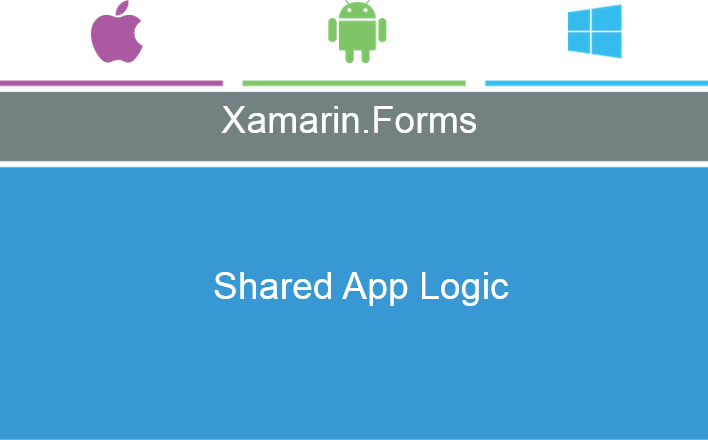
\includegraphics[width=1\textwidth]{images/code-sharing2.png}
		\caption{Xamarin.Forms Architektur (Quelle: https://blog.goyello.com/)}
		\label{fig:xamarinarchitectur}
	\end{figure}

	Abbildung \ref{fig:xamarinarchitectur} zeigt wie die Xamarin.Forms Architektur aussieht. Dabei werden die Nativen Bibliotheken von Android \textit{Android SDK}, iOS \textit{iOS UIKit} und Windows Phone bzw. Windows Mobile \textit{UWP SDK} eingebunden. Das Einbinden dieser Bibliotheken stellt dem Framework eine Vielzahl an UI Elementen zur Darstellung von Inhalten zur Verfügung. In der derzeitigen Version von Xamarin.Forms sind es 17 unterschiedliche Elemente.

	Jedoch ist zu beachten, dass der in Abbildung \ref{fig:xamarinarchitectur} in grau dargestellte Balken den Shared UI Code repräsentiert. Auf diesem aufbauend muss mit ungefähr 20\% Zielplattform spezifischen UI Design gerechnet werden \cite{book:Xamarin-Mobile-Application-Development}. Näheres dazu wird in den folgenden Abschnitten \ref{sec:xamarinformsmvvm} sowie \ref{chap:xamarinformsdevelopment} genauer erläutert.

	Wie Xamarin.Forms das rendern eines UI Elements durchführt ist in Abbildung \ref{fig:xamarinaformsrender} zu erkennen.

	\begin{figure}[h!]
		\centering
		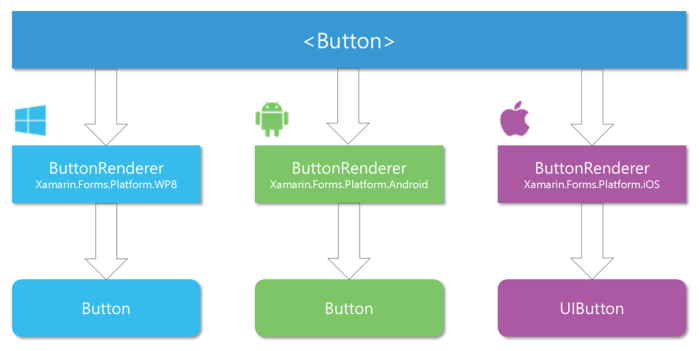
\includegraphics[width=0.9\textwidth]{images/xamarinforms-button-rendering.png}
		\caption[Wie Xamarin UI Elemente rendert]{Wie Xamarin UI Elemente rendert\\\hspace{\textwidth}(Quelle: igorelikblog.wordpress.com/2016/07/08/xamarin-form-memory-management)}
		\label{fig:xamarinaformsrender}
	\end{figure}

	Das Element \textbf{$<$Button$>$} wird im Layout File welches in XAML (Extensible Application Markup Language) geschrieben wurde, eingebaut. Wird der Code nun kompiliert ist der \textit{ButtonRenderer} jener Plattformspezifische renderer der, dass Xamarin.Forms UI Element in Nativen Code umsetzt. Der \textbf{$<$Button$>$} unter Xamarin.Forms wird dadurch in einen \textbf{UIButton} für iOS oder einen \textbf{Android.Button} für Android übersetzt. Dieses rendern macht Xamarin.Form einzigartig, da im Vergleich mit anderen Cross-platform Technologien das Design für die Zielplattformen meist mittels HTML oder CSS vorgenommen werden muss, um die UI Elemente in Native Design Elemente zu transformieren \cite{book:Xamarin-Mobile-Application-Development}.

	\textbf{Rendering} ist der Arbeitsschritt einer Bilderstellung aus Objekten die, wie im Beispiel des Xamarin.Forms Frameworks, aus grafischen Objekten bestehen, welche in XAML definiert wurden\footnote{https://www.itwissen.info/Rendering-rendering.html}.

	\textbf{XAML} ist die Beschreibungssprache die Xamarin verwendet um die grafische Gestaltung des UI zu ermöglichen. Da XAML nur eine Beschreibungssprache ist kann es keinen Code enthalten. Alle Event Handler, wie zum Beispiel das Klicken eines Button, müssen in einem Code File definiert werden.
	test

	\newpage
	Eine Standard XAML Datei ist in Abbildung \ref{fig:xamarinaformxamlpreview} dargestellt. Die Deklarationen in Zeile zwei bis drei definieren das der Namespace von Microsoft verwendet werden soll. In Zeile fünf wir ein Präfix für einen lokalen Namespace definiert um Zuweisungen im XAML File mit dem Code Behind File zu ermöglichen. Wird eine XAML Datei der PCL Klasse hinzugefügt, erzeugt die IDE neben der Layout Datei zusätzlich eine Code behind Datei. Diese ist in Abbildung \ref{fig:xamarinaformxamlpreview} als zweiter Tab zu erkennen. Über die Klasse \textit{MCKBPage.xaml.cs} wird das verhalten der App implementiert. Die Referenzierung erfolgt über die Namespace Deklarationen im XAML File.

	\begin{figure}[h!]
		\centering
		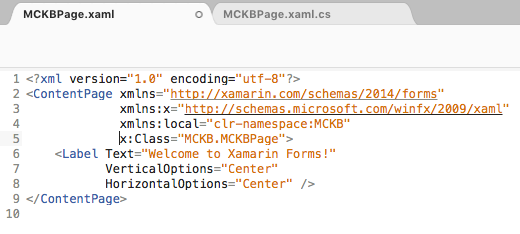
\includegraphics[width=1\textwidth]{images/XAML-preview.png}
		\caption[Aufbau einer XAML Datei für Xamarin.Forms]{Aufbau einer XAML Datei für Xamarin.Forms}
		\label{fig:xamarinaformxamlpreview}
	\end{figure}
	Für die Entwicklung der CP App wird Visual Studio for Mac verwendet, weil somit eine iOS Anwendung einfacher getestet werden kann. Man kann eine iOS App auch mit Windows erstellen, allerdings benötigt man dazu einen Mac im gleichen WLAN Netzwerk damit der Compiler die App erzeugen und ausführen kann.

	\newpage
	\textbf{PCL} steht für Portable Class Library und ist jene Klasse des Projektes in welcher sich der gemeinsame Code für die Cross-platform App befindet.
	
	\begin{figure}[h!]
		\centering
		\begin{minipage}{.4\textwidth}
			\centering
			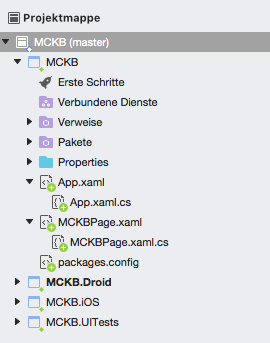
\includegraphics[width=.9\textwidth]{images/project-structure.png}
        	\label{fig:xamarinformprojectstructure}
			\caption[Projekt Struktur einer CP App]{\\\hspace{\textwidth}Projekt Struktur einer CP App}
		\end{minipage}
		\begin{minipage}{.5\textwidth}
			In Abbildung 2.4 sind alle relevanten Klassen aufgelistet die für eine Cross-platform Applikation benötigt werden. Die \textbf{PCL} Klasse ist im Ordner \textit{MCKB} implementiert. Die weiteren Ordner beginnend mit \textit{MCKB.} gefolgt von \textit{Droid} oder \textit{iOS} können dafür verwendet werden gezielt Plattformspezifischen Code zu implementieren welcher nicht von beiden Zielbetriebssystemen verwendet wird. 
        	Weiters ist das XAML File aus Abbildung \ref{fig:xamarinaformxamlpreview} mit dessen Code Behind File zu erkennen. Die Ordner, \textit{Verweise} werden benötigt damit der Compiler die korrekte Zuordnung zum Zielbetriebssystem durchführen kann. Der Ordner \textit{Pakete} ermöglicht es Pakete des \textbf{NuGET} Paket Managers einzubinden. Ein solches Paket kann beispielsweise eine MySQL Anbindung an einen Server sein.
        \end{minipage}
	\end{figure}
	% Die in Abbildung \ref{fig:xamarinformprojectstructure} wird im Laufe der Entwicklung um einige XAML und Code Behind Files wachsen. Der Prozess der Programmierung ist in Abschnitt \ref{chap:xamarinformsdevelopment} festgehalten.
	\newpage

\section{Entwicklung unter Xamarin.Forms}
\label{sec:xamarinformsdevelopement}

	Wie schon in Abschnitt \ref{chap:xamarin} eingangs kurz angeschnitten wurden die Unterschiede der Kompilierung von Xamarin aufgezeigt. Als Entwickler kann man in C\# auf die schon bekannten .NET Klassen, aufgrund von Mono zugreifen und die Applikationslogik implementieren. Ist die App für den ersten Testlauf bereit, wählt man in der Projekt Struktur die Zielplattform aus und markiert diese als Start Projekt. In Abbildung \ref{fig:xamarinformprojectstructure} ist dies zum Beispiel \textit{MCKB.Droid}, da dieser Ordner durch eine Dicke Schrift hervorgehoben wurde.

	Der Prozess der Kompilierung ist in Abbildung \ref{fig:xamarinanativeandroidcompile} zu erkennen.
	\begin{figure}[h!]
		\centering
		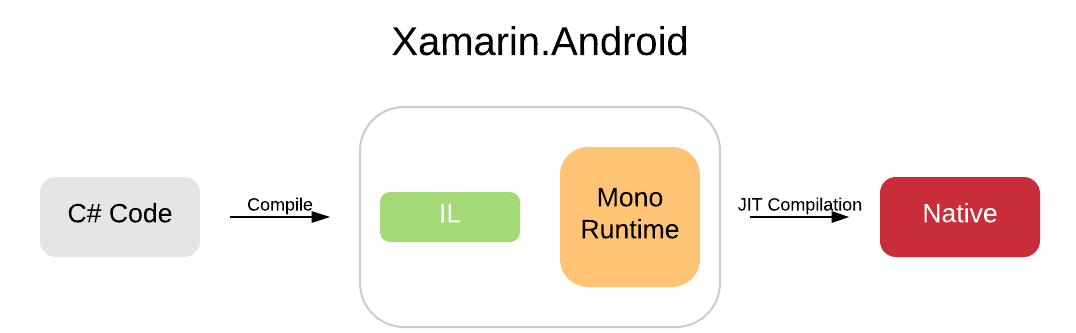
\includegraphics[width=1\textwidth]{images/Xamarin-Android.png}
		\caption{Wie Xamarin.Android kompiliert wird}
		\label{fig:xamarinanativeandroidcompile}
	\end{figure}

	Der C\# Code wird in die Intermediate Language (IL) umgesetzt und in die Mono Runtime geladen. Anschließend übernimmt der Just-In-Time (JIT) Compiler die Übersetzung in Nativen Code der anschließend auf dem Zielbetriebssystem ausgeführt wird. Dieser Prozess läuft im Xamarin Frameworks automatisch ab sobald die Applikation erstellt und auf das Virtuelle oder Hardware Gerät geladen werden soll.

	Wählt man in Abbildung \ref{fig:xamarinformprojectstructure} iOS als Startprojekt, \textit{MCKB.iOS} ist dann Dick hervorgehoben, so sieht der Erstellungsprozess differenzierter aus, da Apple eine JIT Kompilierung nicht unterstützt. Betrachtet man Abbildung \ref{fig:xamarinanativeioscompile} genauer erklärt es warum man einen Apple Computer für die Erstellung einer iOS oder MacOS Anwendung benötigt.
	\begin{figure}[h!]
		\centering
		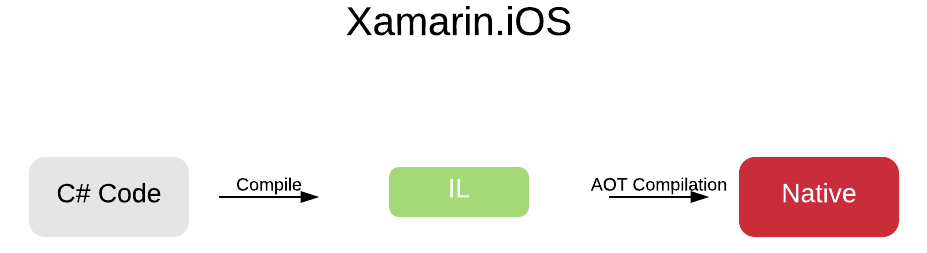
\includegraphics[width=1\textwidth]{images/Xamarin-iOS.png}
		\caption{Wie Xamarin.iOS kompiliert wird}
		\label{fig:xamarinanativeioscompile}
	\end{figure}

	Für die Erstellung der iOS App wird gleich wie bei einer Android App der C\# Code in die IL kompiliert. Da nun keine Mono Runtime zur Verfügung steht wird ein Apple Compiler benötigt. Dieser Compiler ist der Ahead-of-Time (AOT) Compiler der nun die Übersetzung in Nativen Code übernimmt.

	Xamarin.Forms stellt eine höhere Abstraktions Ebene für die Entwicklung einer Applikation dar. Der Kompilierungsprozess lässt sich folgendermaßen darstellen.
	\begin{figure}[h!]
		\centering
		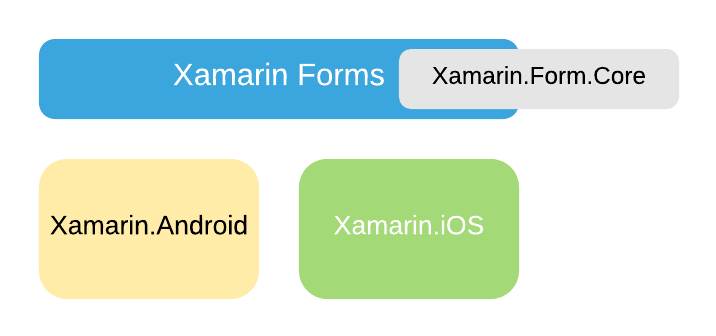
\includegraphics[width=1\textwidth]{images/Xamarin-Forms.png}
		\caption{Xamarin.Forms Architektur}
		\label{fig:xamarinformsarchitecture}
	\end{figure}

	Abbildung \ref{fig:xamarinformsarchitecture} beschreibt was durch Xamarin.Forms erzielt werden soll. Es baut auf den Bibliotheken für die Übersetzung in Nativen Android und iOS Code auf und ist das fehlende Bindeglied für den Prozess in Abbildung \ref{fig:xamarinaformsrender} (Rendering eines Button von Xamarin.Forms). Jener Part der für die Übersetzung des Codes zuständig ist, ist die \textit{Xamarin.Forms.Core} Bibliothek. Die in dem XAML File festgelegten UI Elemente der PCL Klasse sind Teil dieser \textit{Xamarin.Forms.Core} Bibliothek. Der Compiler übersetzt nun für die UI ELemente für Android, siehe Abbildung \ref{fig:xamarinanativeandroidcompile} und iOS, siehe Abbildung \ref{fig:xamarinanativeioscompile}, damit das Zielplattform spezifische Design dargestellt wird.
	\newpage

\subsection{Model View ViewModel - Design/Architectural Pattern}
\label{sec:xamarinformsmvvm}
	
	\textbf{MVVM} ist eine Variante des \textit{Model View Controller Pattern} und dient dazu eine verbesserte Testbarkeit (Unit-Testing) durch Trennung der Benutzerschnittstelle und der sich dahinter befindlichen Logik der Benutzerschnittstelle zu ermöglichen. In einigen Büchern zur Entwicklung mit Xamarin wird auf das MVVM Pattern verwiesen da es eine Architektur Struktur für User Interfaces implementiert\cite{book:Xamarin.Forms-Essentials:}. Dies ist vor allem für komplexe Applikationen von Nutzen da durch eine verbesserte Testbarkeit von Modulen die Benutzerfreundlichkeit erheblich gesteigert werden kann.

	\textbf{Model:} Repräsentiert ein Business Objekt das die Daten und das Verhalten der Applikation kapselt. Für die MCKB Applikation wären dies:
	\begin{itemize}
		\setlength\itemsep{0em}
		\item Artikel
		\item Anwender
		\item Kommentare zu Artikeln
	\end{itemize}

	\textbf{View:} Ist das was der Anwender sieht wenn er die Applikation verwendet. Artikel werden in \textit{Pages\footnote{https://docs.microsoft.com/en-us/xamarin/xamarin-forms/user-interface/controls/pages}} dargestellt. Kommentare, welche Teil einer Artikel Page sind, die es zu Artikeln gibt werden angezeigt und können hinzugefügt werden. Wie der View definiert wird hängt von der Design Spezifizierung der Page und dessen Layout ab und kann Beispielsweise eines folgender Layouts sein:
	\begin{itemize}
		\setlength\itemsep{0em}
		\item Content Page
		\item Navigation Page
		\item Tabbed Page
		\item Carousel Page
		\item ...
	\end{itemize}
	Innerhalb einer Page kann ein Layout definiert werden um Daten nach einem Schema darzustellen. Folgende \textit{Layouts\footnote{https://docs.microsoft.com/en-us/xamarin/xamarin-forms/user-interface/controls/layouts}} kann eine Page enthalten:
	\begin{itemize}
		\setlength\itemsep{0em}
		\item Content View
		\item Scroll View
		\item Stack, Absolute, Relative oder Grid Layout
	\end{itemize}

	\textbf{ViewModel:} Dies ist ein Model welches für einen View entworfen wurde. Es ist eine Klasse mit Eigenschaften welche den Zustand eines View's sowie Methoden und die Logik eines View's implementiert.
	\newpage
	Ein ViewModel für den View in Codeabschnitt \ref{lst:xamarinmvvmview}, welches eine \textit{Page} mit einem \textit{Stacklayout (horizontale Anordnung von UI Elementen)}, einem \textbf{Button} und einen \textbf{ListView} mit \textbf{Items} enthält, hätte beispielsweise ein ViewModel, welches in Codeabschnitt \ref{lst:xamarinmvvmviewmodel} abgebildet ist, um Elemente dem ListView hinzuzufügen:\\

	\begin{lstlisting}[caption={Beispiel View},label={lst:xamarinmvvmview},captionpos=b,style=JAVA-Own]
<?xml version="1.0" encoding="utf-8"?>
<ContentPage xmlns="http://xamarin.com/schemas/2014/forms"
             xmlns:x="http://schemas.microsoft.com/winfx/2009/xaml"
             xmlns:local="clr-namespace:MCKB" x:Class="MCKB.MCKBPage">
    <StackLayout>
        <Button Text="Add"/>
        <ListView x:Name="ArticleView">
        <ListView.ItemTemplate>
          <DataTemplate>
            <TextCell Text="{Binding ArtcleName}" />
          </DataTemplate>
        </ListView.ItemTemplate>
      </ListView>
    </StackLayout>
</ContentPage>
	\end{lstlisting}

	\begin{lstlisting}[caption={Beispiel ViewModel für Codeabschnitt \ref{lst:xamarinmvvmview} (View)},label={lst:xamarinmvvmviewmodel},captionpos=b,style=csharp]
class ViewModel{
	ObservableCollection Item;
	void Add(){
		//Implement function here
	}
}
	\end{lstlisting}

	Auf den Ersten Blick sieht das ViewModel in Codeabschnitt \ref{lst:xamarinmvvmviewmodel} aus wie eine code-behind Implementierung (der Button wird mit einem Event-Handler verlinkt um die Add Funktion aufzurufen) für das XAML des View in Codeabschnitt \ref{lst:xamarinmvvmview} aus. Jedoch ist ein ViewModel keine code-behind Implementierung.

	\textbf{Code-behind} ist fest an Xamarin gekoppelt. Dies führt dazu, dass es schwer ist für eine solche code-behind Klasse einen Unit-Test zu implementieren. Um den Code in der code-behind Klasse dennoch testen zu können wird dieser Code in die ViewModel Klasse geschrieben und abgeändert um eine minimale Kopplung mit Xamarin zu haben. Der Code ist nun ein \textbf{Plain Old CLR Object (POCO)} Objekt für das Unit-Tests erzeugt werden können.

	\textbf{Unit/Model Tests} sind Software Tests welche funktionale Einzelteile von Software auf deren korrekte Funktionalität testen. Die für diese Arbeit geschriebene Cross-platform Applikation wird keine Unit/Modul Test implementieren.

\newpage
\subsection{Projekterstellung mit Visual Studio for Mac}
\label{sec:xamarincreateproject}

	Für die Entwicklung der Cross-Platform Applikation wird \textbf{Visual Studio for Mac} verwendet im sowohl eine Android als auch iOS Version der Applikation entwickeln zu können. Die Projekterstellung unter Windows mit \textbf{Visual Studio 2015} oder \textbf{2017} verläuft analog im gleichen Schema.

	Zu Beginn wird eine Standard Xamarin.Forms Applikation erstellt. Hierbei muss entschieden werden wie der Cross-Platform Code geteilt werden soll:

	\begin{figure}[h!]
		\centering
		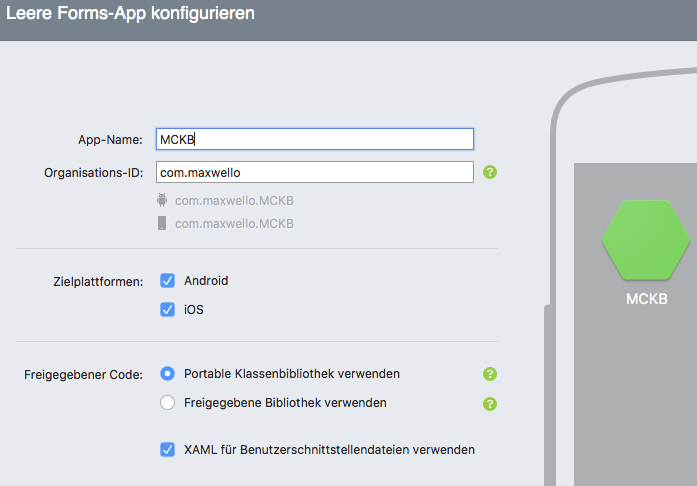
\includegraphics[width=1\textwidth]{images/Project-Setup-one.png}
		\caption{Erstellung der Xamarin.Forms App - MCKB}
		\label{fig:xamarinprojectstart}
	\end{figure}

	In Abbildung \ref{fig:xamarinprojectstart} ist zu erkennen das schon bei der Erstellung der Applikation festgelegt werden muss auf welche Art und Weise der \textit{Shared Code}, der CP-App implementiert werden soll.

	In Abbildung \ref{fig:xamarinsharedcode} ist zu erkennen wie sich \textbf{Portable Class Library} von \textbf{Shared Library} unterscheiden. Wird PCL für den freigegeben Code verwendet, siehe Abbildung \ref{fig:xamarinsharedcode} links, so erstellt die IDE alle notwendigen Verweise und verlinkt diese. Anders ist dies bei einem Shared Library (SL) Projekt, bei welchem der Entwickler selbst die notwendigen Verweise zu weiteren dependencies einbinden muss.

	\newpage
	\begin{figure}[h!]
		\centering
		\begin{subfigure}
			\centering
			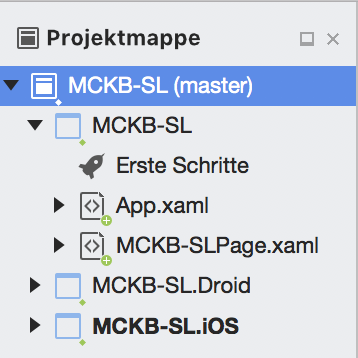
\includegraphics[width=.3\textwidth]{images/xamarin-shared-library.png}
		\end{subfigure}
		\begin{subfigure}
			\centering
			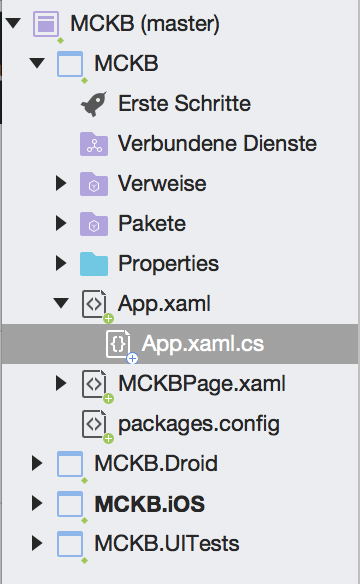
\includegraphics[width=.3\textwidth]{images/xamarin-portable-class.png}
		\end{subfigure}
		\caption{Unterschied Shared Code - Xamarin.Forms App - MCKB}
		\label{fig:xamarinsharedcode}
	\end{figure}

	Der Unterschied auf welche Art und Weise der freigegebene Code für die Applikation verwaltet werden soll muss von Beginn an definiert werden. Eine Änderung im Nachhinein ist nicht mehr möglich.

	\textbf{Eine Portable Klassenbibliothek (\textit{PCL})} erstellt wie schon erwähnt alle notwendigen Verweise für eine Android und iOS Cross-Plattform Applikation. Dabei spielen die folgenden Verweise eine wichtige Rolle:
	\begin{itemize}
		\setlength\itemsep{0em}
		\item \textit{Xamarin.Forms.Core} definiert eine allgemeine API (Application Programming Interface) für Klassen wie zum Beispiel Buttons, Labels, ListViews uvm.
		\item \textit{Xamarin.Forms.Platform} linkt die Plattform spezifischen Renderer von Android und iOS damit Elemente in der PCL Klasse in Plattform spezifischen Code übersetzt werden können.
		\item \textit{Xamarin.Forms.Xaml}
	\end{itemize}
	Der Code in einer PCL wird zur Laufzeit zu einer \textit{dynamically-linked library (DLL)} für die Zielplattform Referenzen zusammengefasst. Ist es für die Cross-platform Applikation notwendig Nativen Code auszuführen, kann dies durch bestimmte \textbf{IF Abfragen} in der PCL Klasse umgesetzt werden.\\

	\begin{lstlisting}[caption={Plattform spezifischen Code in PCL ausführen},label={lst:xamarinpcl},captionpos=b,style=csharp]
...
if (Device.OS == TargetPlatform.iOS){
	//Run iOS Code here..
}
...
else if (Device.OS == Target.Platform.Android){
	//Run Android Code here...
}
...
	\end{lstlisting}

	\textbf{Die Freigegebene Bibliothek (\textit{Shared Library (SL)/Shared Asset (SA)})\footnote{https://docs.microsoft.com/en-us/xamarin/cross-platform/app-fundamentals/code-sharing}} stellt den einfachsten Ansatz für \textit{Code Sharing} dar. Für die Zielplattform wird nur jener Code dementsprechend kompiliert wenn es die dafür notwendigen Präprozessor Anweisungen enthält. Es wird somit der gesamte Inhalt des Projektes in jeden referenzierenden Teil des Projektes kopiert, als wäre es ein Teil davon.\\

	\begin{lstlisting}[caption={Plattform spezifischen Code in SA/SL ausführen},label={lst:xamarinslsa},captionpos=b,style=csharp]
#if __iOS__
	//Run iOS Code here..
...
#elif __ANDROID__
	//Run Android Code here...
...
#endif
	\end{lstlisting}

	Codeabschnitt \ref{lst:xamarinslsa} veranschaulicht diese Präprozessor Anweisungen die in den C\# Klassen den Plattformspezifischen Code zu finden sind.

	Wird eine PCL als Code Sharing Basis verwendet. wird der Zugriff auf mögliche \textit{.NET Klassen} auf eine kleinere Untermenge beschränkt, jedoch kann dieses Problem durch Implementierung einer Schnittstelle, da dadurch auf die Ursprüngliche Menge an .NET Klassen zurückgegriffen werden kann.



















